\documentclass{article}
\title{Physics 247 HW 13}
\author{Name: Hleb Zhynko}
\date{Due: December 12, 2022}

\usepackage{amsmath}
\usepackage{graphicx}

\graphicspath{ {./figures} }

\begin{document}

\maketitle

\section*{Problem 1}
Let $\tau = I\alpha$ be the torque of the bar, $\alpha$ - the final instantaneous angular acceleration of the bar, and $I = \frac{1}{3}ML^2$ - the moment of inertia of the bar.

\[
\tau = F \times r = Mg\sin{30^{\circ}} \times r = Mg\sin{30^{\circ}} \times \frac{L}{2};
\]
\[
\alpha = \frac{Mgr\sin{30^{\circ}}}{\frac{1}{3}ML^2} = \frac{3}{2}\frac{1}{2}\frac{g}{L} = \frac{3}{4}\frac{g}{L}.
\]

\section*{Problem 2}
Let $H = L\cos{30^{\circ}}$ be the change in height of the tip of the bar. Using conservation of energy:

\[
MgH = \frac{1}{2}I\omega^2;
\]
\[
MgL\cos{30^{\circ}} = \frac{1}{2}\frac{1}{3}ML^2\omega^2;
\]
\[
\omega^2 = \frac{1}{L}6g\frac{\sqrt{3}}{2};
\]
\[
\omega = \sqrt{\frac{3\sqrt{3}g}{L}};
\]
\[
v = \omega R = \omega L = \sqrt{3\sqrt{3}gL}.
\]

\section*{Problem 3}
Using conservation of energy for all three cases:

For the cube:
\[
\frac{1}{2}Mv^2 = Mgh;
\]
\[
h = \frac{v^2}{2g}.
\]

For the hoop and the disk:
\[
\frac{1}{2}I\frac{v}{r}^2 + \frac{1}{2}Mv^2 = Mgh;
\]
\[
\frac{v^2}{2}\left(\frac{I}{r^2} + M\right) = Mgh;
\]
\[
h = \frac{v^2}{2Mg}\left(\frac{I}{r^2} + M\right).
\]

For the hoop:
\[
\begin{cases}
I = Mr^2,\\
h = \frac{v^2}{2Mg}\left(\frac{I}{r^2} + M\right);
\end{cases}
\]
\[
h = \frac{v^2}{g}.
\]

For the disk:
\[
\begin{cases}
I = \frac{1}{2}Mr^2,\\
h = \frac{v^2}{2Mg}\left(\frac{I}{r^2} + M\right);
\end{cases}
\]
\[
h = \frac{3}{4}\frac{v^2}{g}.
\]

Assuming the initial velocity $v$ is the same across all three cases, the hoop will get to the highest point.

\section*{Problem 4}
\begin{figure}
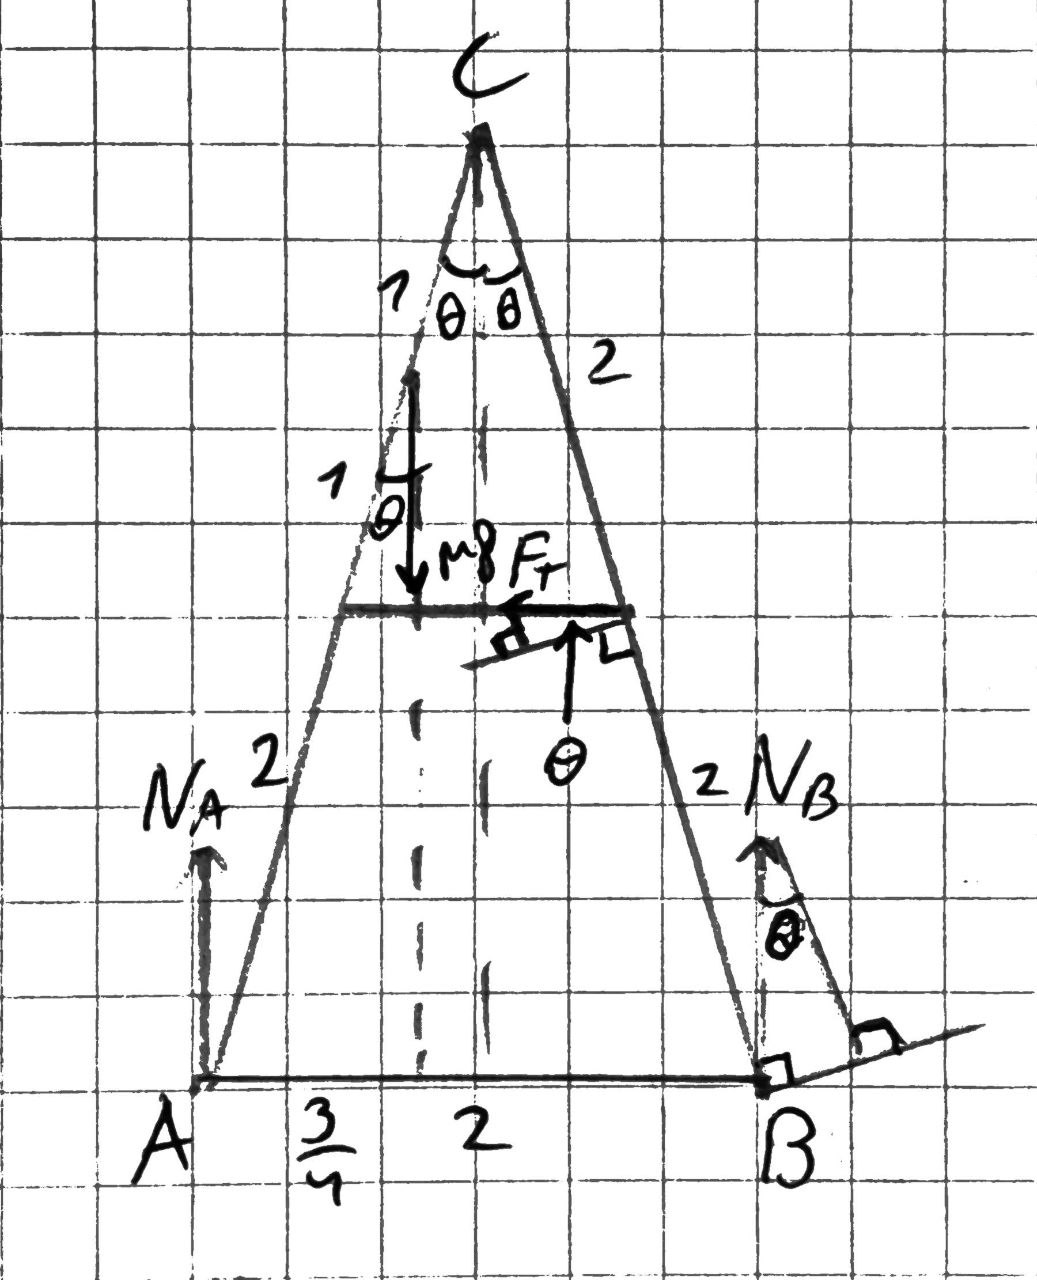
\includegraphics[scale=0.3]{p4fig1}
\centering
\caption{A diagram of the step ladder.}
\label{fig:diagram}
\end{figure}

See Figure \ref{fig:diagram} for the diagram of the problem. Let $\tau_A$ be the torque at point A, and $\tau_{Cright}$ - the torque of the right half of the ladder at point C.

\[
\sin{\theta} = \frac{1}{4}; \cos{\theta} = \frac{\sqrt{15}}{4};
\]
\[
\tau_A = -\frac{3}{4}mg + 2N_B = 0; \Rightarrow N_B = \frac{3}{8}mg;
\]
\[
\tau_{Cright} = -2F_T\cos{\theta} + 4N_B\sin{\theta} = 0; \Rightarrow N_B = 2\frac{\sqrt{15}}{4}F_T;
\]
\[
\frac{3}{8}mg = 2\frac{\sqrt{15}}{4}F_T;
\]
\[
F_T = \frac{3}{4}\frac{1}{\sqrt{15}}mg \approx 132.98\,N.
\]

\end{document}